\chapter{Fundamentals}
\label{ch:method} % Label for method chapter
In this chapter, I explore the foundational concepts that are critical to addressing fine-grained image classification problem.

\section{ General Aspects}
This problem is considered one of fine-grained image classification, because it focuses on distinguishing between classes with very similar features. I was aware that with classic methods of machine learning it would be impossible to develop a good solution.\\[0.2cm]
\noindent
Most documents available online explored the use of convolutional neural networks (CNN), since they are the most viable for problems which involve large quantities of complex data from which features like form and color must be obtained to get accurate results.\\[0.2cm]
\noindent
In both the models I created, the loss function used is Categorical Cross-Entropy (Softmax loss) which is common for multi-class classification. The optimizer is Adam, an implementation of stochastic gradient descent, used with a default learning rate of 0.001. This parameter is one of the hyper-parameters varied during the hyper-parameter tuning phase. I chose accuracy as the metric to evaluate the model performance during training and tuning.\\

\section{Simple Neural Network Architecture}
I decided to try a simple architecture, not applying the concept of transfer learning, but that still could be considered deep learning.\\
It is composed of the following layers (in order):
\noindent
\begin{itemize}
    \item \textbf{Flatten Layer:} This layer flattens the input of shape (299, 299, 3) into a single-dimensional vector with 268,203 elements, preparing the data for the fully connected layers.

    \item \textbf{Dense Layer:} A fully connected layer with 256 neurons and \textbf{ReLU} activation. This activation function maps negative inputs to 0 and leaves positive inputs unchanged, making it suitable for deep learning.

    \item \textbf{Dropout Layer:} A dropout layer with a rate of 0.25, which randomly ignores a fraction of the outputs from the previous layer to prevent overfitting.

    \item \textbf{Batch Normalization Layer:} This layer normalizes the output of the previous layer to have a mean of 0 and a standard deviation of 1, stabilizing and accelerating the training process.

    \item \textbf{Second Dense Layer:} A fully connected layer with 128 neurons and \textbf{ReLU} activation. Similar to the first dense layer, it helps learn complex features.

    \item \textbf{Dropout Layer:} Another dropout layer with a rate of 0.35, further regularizing the model and reducing overfitting.

    \item \textbf{Output Dense Layer:} A fully connected layer with 37 neurons, each representing a classification class. A \textbf{SoftMax} activation function is applied to output a probability distribution over the classes.
\end{itemize}
Fig. 3.1 shows an automatically generated diagram of the architecture of this network.
\begin{figure}[h]
    \centering
    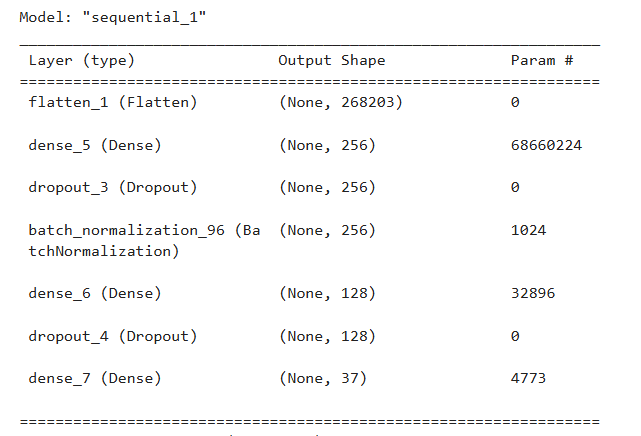
\includegraphics[width=0.7\textwidth]{figures/simple model architecture.png}
    \caption{Automatically generated diagram of the architecture of the simple neural network.}
    \label{fig:architecture_diagram}
\end{figure}

\section{Complex Neural Network Architecture}
As previously mentioned, transfer learning plays a significant role in optimizing new models. In this, pre-trained models are used as the foundation, improving performance for the new task. To achieve this, additional layers are added after the frozen layers of the base model, preventing the destruction of the learned features. These new layers focus on training with the new dataset features and making predictions.

The \textbf{InceptionV3} architecture, pre-trained on the ImageNet dataset, was chosen as the base model because it has been proven effective for similar problems in multiple studies.

This Neural Network combines the following layers:
\begin{itemize}
    \item \textbf{Input Layer:} The first layer that processes the input image with a shape of $(299, 299, 3)$, ensuring it is compatible with the base model. It preprocesses the image by rescaling pixel values to a range between -1 and 1.
    
    \item \textbf{InceptionV3 Base Model:} The pre-trained InceptionV3 network is used without its top layers. All its layers are frozen to preserve the pre-trained features.
    
    \item \textbf{Global Average Pooling Layer:} This layer reduces the dimensions of the feature maps from the base model by averaging their values, resulting in a 1D vector representation.
    
    \item \textbf{Dense Layer (256 units):} A fully connected layer with 256 neurons and ReLU activation to learn new patterns from the extracted features.
    
    \item \textbf{Dropout Layer:} Dropout is applied to randomly ignore 35\% of the neurons, helping prevent overfitting.
    
    \item \textbf{Batch Normalization Layer:} Normalizes the output of the previous layer, stabilizing training and speeding up convergence.
    
    \item \textbf{Output Dense Layer (37 units):} The final layer with 37 neurons, one for each class, using a SoftMax activation function to produce a probability distribution over the classes.
\end{itemize}
 \begin{figure}[h]
    \centering
    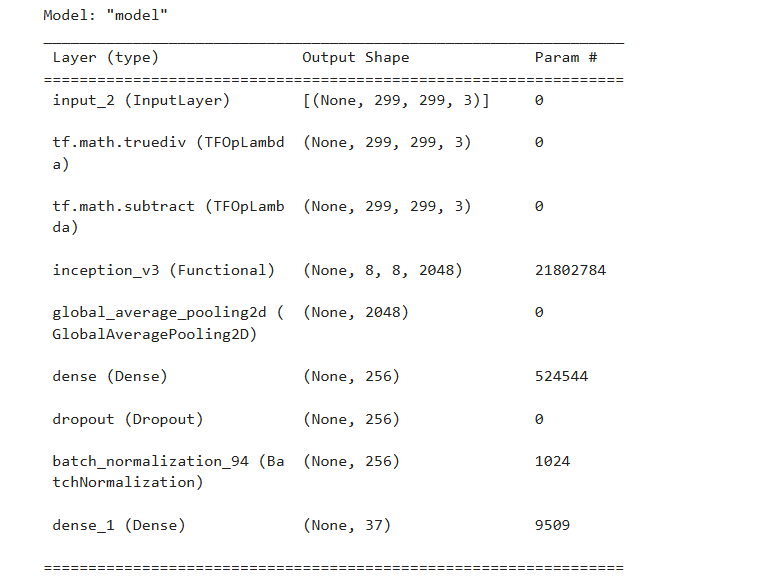
\includegraphics[width=0.7\textwidth]{figures/complex model architecture.png}
    \caption{Automatically generated diagram of the architecture of the complex neural network.}
    \label{fig:example_images}
\end{figure}

\section{Summary}
In this chapter, I explained the key concepts and methods used for solving the fine-grained image classification problem. I discussed the use of convolutional neural networks (CNNs) for handling complex image data and described two architectures: a simple neural network and a more advanced model using transfer learning with the InceptionV3 architecture. Important components like pre-processing, dropout, batch normalization, and activation functions (ReLU and SoftMax) were also highlighted.


